\section{Tujuan}
\begin{itemize}[label=$\bullet$, itemsep=-1pt, leftmargin=*]   
    \item Mahasiswa mengerti tentang konsep pointer pada bahasa pemrograman C.
    \item Mahasiswa mengerti cara membuat dan memanggil struct pada bahasa pemrograman C.
    \item Mahasiswa mengerti tentang algoritma sorting pada bahasa pemrograman C.
    \item Mahasiswa mengerti tentang algoritma searching pada bahasa pemrograman C.
    \item Mahasiswa mampu mengaplikasikan konsep algoritma searching dan sorting pada bahasa pemrograman C.
\end{itemize}

\section{Pointer}
\subsection{Alamat Memori}
Setiap variabel, fungsi, struct, ataupun objek lain yang dibuat dalam program mempunyai lokasi masing-masing pada memori. Alokasi setiap variabel disimpan dalam alamat memori tertentu.

Jika  terdapat variabel \verb|var| di program Anda, \verb|&var| akan memberi alamatnya di memori.
\begin{lstlisting}[language=c]
    int var = 5;
    printf("%d\n", var);
    printf("%p\n", &var);
\end{lstlisting}
\begin{center}
	\colorbox{pink}{\parbox{0.8\linewidth}{\textbf{Catatan:} Output bisa berbeda-beda di tiap eksekusi.}}
\end{center}

\subsection{Pengenalan Pointer} 

Pointer (variabel penunjuk) adalah variabel khusus yang digunakan untuk menyimpan alamat, bukan nilai.

Deklarasi variabel pointer menggunakan operator \verb|*| di antara tipe data dan nama variabelnya.
\begin{lstlisting}[language=c]
	#include <stdio.h>
int main()
{
	int* p; // atau
    int * p2;
	return 0;
}
\end{lstlisting}


\subsection{Cara Kerja Pointer}
Berikut adalah cara kerja dari pointer.
\begin{lstlisting}[language=c, caption={Contoh Program Pointer}]
    #include <stdio.h>
    int main()
    {
       int* pc, c;
       
       c = 22;
       printf("Address of c: %p\n", &c);
       printf("Value of c: %d\n\n", c);  // 22
       
       pc = &c;
       printf("Address of pointer pc: %p\n", pc);
       printf("Content of pointer pc: %d\n\n", *pc); // 22
       
       c = 11;
       printf("Address of pointer pc: %p\n", pc);
       printf("Content of pointer pc: %d\n\n", *pc); // 11
       
       *pc = 2;
       printf("Address of c: %p\n", &c);
       printf("Value of c: %d\n\n", c); // 2
       return 0;
    }
\end{lstlisting}

Penjelasan Program:\\
\begin{enumerate}
    \item \verb|int* pc, c;|
    \begin{figure}[H]
        \centering
        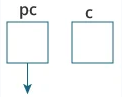
\includegraphics[width=0.2\linewidth]{../P4/img/screenshot001.png}
        \caption{}
        \label{fig:satu}
    \end{figure}
    \item \verb|c = 22;|
    \begin{figure}[H]
        \centering
        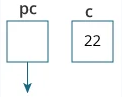
\includegraphics[width=0.2\linewidth]{../P4/img/screenshot002.png}
        \caption{}
        \label{fig:dua}
    \end{figure}
    \item \verb|pc = &c;|
    \begin{figure}[H]
        \centering
        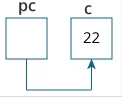
\includegraphics[width=0.2\linewidth]{../P4/img/screenshot003.png}
        \caption{}
        \label{fig:tiga}
    \end{figure}
    \item \verb|c = 11;|
    \begin{figure}[H]
        \centering
        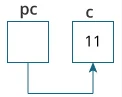
\includegraphics[width=0.2\linewidth]{../P4/img/screenshot004.png}
        \caption{}
        \label{fig:empat}
    \end{figure}
    \item \verb|*pc = 2;|
    \begin{figure}[H]
        \centering
        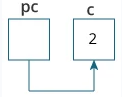
\includegraphics[width=0.2\linewidth]{../P4/img/screenshot005.png}
        \caption{}
        \label{fig:lima}
    \end{figure}
\end{enumerate}

\subsection{Double Pointer}
Variabel pointer juga dapat menunjuk variabel pointer lainnya. 
Hal ini disebut dengan double pointer (pointer to pointer). 
Untuk mendeklarasikan variabel double pointer, digunakan dua simbol *. 
Kegunaan paling umum dari variabel double pointer adalah untuk membuat array dua dimensi secara dinamis.
\begin{lstlisting}[language=c]
    int **dbPtr;
\end{lstlisting}
Variabel dbPtr di atas menyimpan alamat memori dari variabel pointer lainnya. \\
Berikut contohnya
\begin{lstlisting}[language=c,  caption={Contoh Double Pointer}]
#include <stdio.h>

int main(void)
{
    int var = 23;
    int *ptr = &var;
    int **dbPtr = &ptr;

    printf("%d\n", **dbPtr);
        
    return 0;
}
\end{lstlisting}

\subsection{Tugas Pendahuluan}
\begin{enumerate}
   \item Bagaimana cara mendeklarasikan pointer ke array multidimensi?
   \item Buatlah program dalam bahasa C atau C++ yang mengimplementasikan 
   fungsi void printMatrix(int **matrix, int rows, int cols) untuk mencetak matriks 2D menggunakan pointer ke pointer. Lalu, dalam fungsi main, 
   buatlah matriks 2D dan panggil fungsi printMatrix untuk mencetak matriks tersebut.
\end{enumerate}

\section{Struct}
Dalam pemrograman C, struct (atau struktur) adalah kumpulan variabel (bisa dari tipe berbeda) di bawah satu nama. 
Tidak seperti array yang hanya dapat menyimpan elemen dengan tipe data sama, 
struct dapat mengelompokkan elemen dengan tipe data yang berbeda-beda.


\subsection{Deklarasi Struct}
Seperti variabel, struct harus dideklarasikan terlebih dahulu sebelum bisa digunakan. Pendeklarasian struct menggunakan sintaks sebagai berikut.

\begin{lstlisting}[language=c]
struct <nama_struct> {
    <tipe_data_member> <nama_member>;
    <tipe_data_member> <nama_member>;
    <tipe_data_member> <nama_member>;
    .
    .
    .
};
\end{lstlisting}

Berikut adalah contoh deklarasi struct berdasarkan kasus Mahasiswa.
\begin{lstlisting}[language=c]
struct Mahasiswa
{
    char *name;
    char *address;
    int age;
};
\end{lstlisting}
\begin{center}
	\colorbox{pink}{\parbox{0.8\linewidth}{\textbf{Catatan:}  Menggunakan pointer * untuk data string}}
\end{center}

Setelah dideklarasikan, sebuah struct akan menjadi tipe data baru. 
Maka dalam kasus ini, struct Mahasiswa di sini menjadi tipe data baru dengan member-member berupa \verb|nama|, \verb|address|, dan \verb|age|. 
Untuk membuat variabel dengan tipe data struct, dilakukan dengan sintaks berikut.

\begin{lstlisting}[language=c]
    struct <nama_struct> <nama_variabel>;
\end{lstlisting}

Contoh:
\begin{lstlisting}[language=c]
    struct Mahasiswa mhs1;
    struct Mahasiswa mhs2;
\end{lstlisting}
Contoh di atas menunjukkan terdapat dua variabel \verb|mhs1| dan \verb|mhs2 |bertipe struct \verb|Mahasiswa|.

\subsection{Akses Member Struct}
Bagaimana cara untuk mengakses member dari variabel struct yang telah dibuat? \\
Untuk mengakses member-member dari struct, digunakan operator dot (.) setelah nama variabelnya.
\begin{lstlisting}[language=c]
    <nama_variabel>.<member_struct>
\end{lstlisting}

Contoh:
\begin{lstlisting}[language=c]
    mhs1.age = 20;
    mhs1.nama = iqbal;
    
    mhs2.nama = fatur;
    mhs2.age = 21;
\end{lstlisting}

\subsection{Tugas Pendahuluan}
\begin{enumerate}
    \item Buatlah sebuah struct yang merepresentasikan informasi tentang seorang mahasiswa, yang memiliki nama, nim, dan nilai IPK. Kemudian, buatlah program untuk menginput data mahasiswa, menampilkan data mahasiswa, dan menghitung rata-rata IPK dari sejumlah mahasiswa.
    \item Anda diberikan struct yang merepresentasikan titik dalam sistem koordinat dua dimensi (x, y). Buatlah sebuah program C untuk menghitung jarak antara dua titik yang diinputkan oleh pengguna menggunakan rumus jarak Euclidean.
\end{enumerate}

\section{Algoritma Sorting}
Sorting merupakan suatu proses penyortiran atau pengurutan sebuah data.\\
Terdapat 2 macam pengurutan data pada sorting yaitu :
\begin{enumerate}
    \item Berdasarkan ascending (kecil ke besar).
    \item Berdasarkan Descending (besar ke kecil).
\end{enumerate}

\subsection{Bubble Sort}
Bubble sort merupakan algoritma pengurutan yang membandingkan dua data yang berdekatan dan menukarnya sampai tidak dalam urutan yang diinginkan.
Bubble sort menggunakan teknik iterasi. Iterasi merupakan proses melakukan perulangan sebanyak data yang diketahui.
Intinya pada iterasi melakukan perbandingan antara dua data.

\begin{figure}[H]
    \centering
    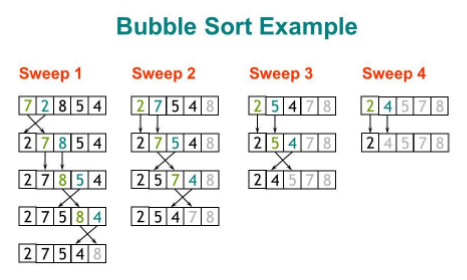
\includegraphics[width=0.7\linewidth]{../P4/img/screenshot006.png}
    \caption{}
    \label{fig:enam}
\end{figure}

\begin{lstlisting}[language=c,caption=Implementasi Bubble Sort]
void swap ( int * xp , int * yp ) {
   int temp = *xp;
   *xp = *yp;
   *yp = temp;
}

void bubbleSort(int arr[], int n) {
   int i, j, swapped;        // dioptimasi dengan bool `swapped`:
   for (i = 0; i < n-1; i++) {
      swapped = 0;
      for (j = 0; j < n-i-1; j++) {
         if (arr[j] > arr[j+1]) {
            swap(&arr[j], &arr[j+1]);
            swapped = 1;
         }
      }
      if (swapped == 0)
         break;
   }
}
\end{lstlisting}

\subsection{Insertion Sort}
Insertion sort merupakan teknik sorting dengan cara menyisipkan atau memasukan setiap elemen secara berulang berulang.
Konsep insertion sort bisa diibaratkan sebuah kartu. 

\begin{figure}[H]
    \centering
    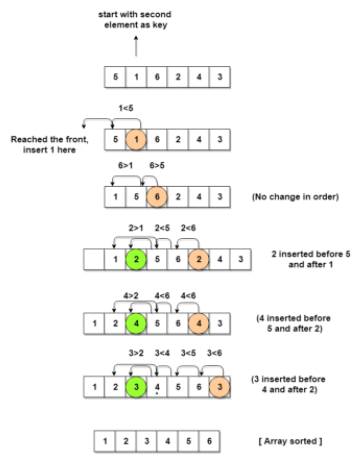
\includegraphics[width=0.5\linewidth]{../P4/img/screenshot007.png}
    \caption{}
    \label{fig:tujuh}
\end{figure}
\begin{lstlisting}[language=c,caption=Implementasi Insertion Sort], 
void insertionSort(int arr[]. int n) {
   int i, key, j;
   for (i = 1; i < n; i++) {
      key = arr[i];
      j = i-1;
    
      while (j >= 0 && arr[j] > key) {
         arr[j+1] = arr[j];
         j = j-1;
      }
      arr[j+1] = key;
   }
}
\end{lstlisting}

\begin{center}
	\colorbox{pink}{\parbox{0.8\linewidth}{\textbf{Catatan:} Terdapat berbagai algoritma sorting lain. Pelajari secara mandiri}}
\end{center}

\subsection{Tugas Pendahuluan}
\begin{enumerate}
    \item Urutkan array berikut menggunakan algoritma Bubble Sort:

    Array: [5, 2, 9, 1, 5, 6]
    \item Hitung kompleksitas waktu (Big O) dari algoritma Insertion Sort saat mengurutkan sebuah array dengan panjang n, dan jelaskan bagaimana kompleksitas ini dihitung.
\end{enumerate}

\section{Algoritma Searching}
Searching merupakan proses pencarian sebuah data yang diinginkan.

\subsection{Linear Search}
Linear Search bekerja dengan melakukan pengecekan kepada semua elemen yang ada.\\
Secara garis besar, cara kerja Linear Search adalah:

\begin{enumerate}
    \item Memeriksa item satu per satu.
    \item Apabila ditemukan, maka “ketemu”.
    \item Jika sampai akhir belum ditemukan, maka item yang dicari tidak ada.
\end{enumerate}

\begin{lstlisting}[language=c,caption=Implementasi Linear Search], 
int linearSearch(int arr[], int n, int item) {
    int i;
    for(i = 0; i < n; ++i) {
        if(item == arr[i])
          return 1;
    }
    return -1;
}
\end{lstlisting}   

\subsection{Binary Search}
Binary Search adalah teknik pencarian di mana untuk setiap iterasinya kita membagi space pencarian menjadi hanya setengah 
dari space pencarian awal hingga kita menemukan yang kita cari.    

\begin{lstlisting}[language=c,caption=Implementasi Binary Search],   
bool f(int k, int a, int b, int n) {
   return ((k/a) * (b/a) >= n);
}

int binser(int a, int b, int n) {
   int l = 1;
   int r = 100000;
   while (r - l > 1) {
      int mid = (l + r) >> 1;
      bool can = f(mid);
      if(can)
         r = mid;
      else
         l = mid + 1;
   }
   if (can(l))
      return l;
   else
      return r;
}
\end{lstlisting}

\begin{center}
	\colorbox{pink}{\parbox{0.8\linewidth}{\textbf{Catatan:} Terdapat berbagai algoritma searching lain. Pelajari secara mandiri}}
\end{center}

\subsection{Tugas Pendahuluan}
\begin{enumerate}
    \item Anda memiliki daftar nama berikut: ["Alice", "Bob", "Charlie", "David", "Eve", "Frank"]. 
    Gunakan algoritma binary search untuk mencari apakah nama "Eve" ada dalam daftar ini. 
    Jika ya, berapa langkah yang dibutuhkan?
    \item Jelaskan perbedaan antara pencarian linear (sequential search) dan pencarian biner (binary search).
     Kapan Anda akan memilih salah satu metode ini daripada yang lain?
\end{enumerate}
